\chapter{Related Work}
\label{chap:relatedWork}

There are a lot of algorithms which focus on image similarity and key feature detection, our main goal being to select specific ones on which we can control the sensitivity of the matches, but also which can be easily and efficiently distributed on several machines for a large input set. \\
We have focused on two main algorithms, the $Harris\ corner\ detector$ and the $Scale\ Invariant$ $Feature\ Transform$.


\section{Harris Corner Detection}

The main idea of the $Harris\ corner\ detector$ \cite{harrisCorner}, \cite{harrisCorner2} algorithm is that, given an input image, the most predominant features that a human eye recognizes and memorizes are corners. A corner is considered to be an intersection of two edges, so, selecting a small area around the point and shifting it should result in a large variation in the intensity of the pixels in that area. \\
Therefore, each area in an image can be classified in three categories:
\begin{itemize}
	\item flat, in which intensities do not vary in either direction (as see in Figure~\ref{fig:flatArea})
	\item edge, in which intensities don't vary in the direction of the edge (as see in Figure~\ref{fig:edgeArea})
	\item corner, in which intensities vary in all directions (as see in Figure~\ref{fig:cornerArea})
\end{itemize}

In order to determine in which category a certain area with a size of $(w, h)$ belongs to, we will compute the variation of intensity: $E(w, h) = \sum_{x, y} w(x, y) * [I(x + w, y + h) - I(x, y)]^2$, where $w$ is a window function, which assigns weights to pixels, and $I$ is the intensity of a certain pixel of the grayscale image.\\
In order to determine the corner areas, we have to maximize the function $\sum_{x, y}[I(x + w, y + v) - I(x, y)]^2$, which using $Taylor$ expansion and representing in a matrix form can be written as
$E(w, h) \approx
\begin{bmatrix}
w & h
\end{bmatrix} * 
\left(\sum_{x, y}
\begin{bmatrix}
I_x^2 & I_xI_y\\
I_xI_y & I_y^2
\end{bmatrix}
\right) *
\begin{bmatrix}
w \\
h
\end{bmatrix}$, and, furthermore, using a substitution
$E(w, h) \approx
\begin{bmatrix}
w & h
\end{bmatrix} * 
M *
\begin{bmatrix}
w \\
h
\end{bmatrix}$.\\
Using this equation, the score of a certain area is computed as $R = det(M) - k * (trace(M))^2$. A higher score of $R$ denotes a higher probability of the area being a corner.

\begin{figure}[ht!]
\centering
\begin{minipage}{.5\textwidth}
	\centering
	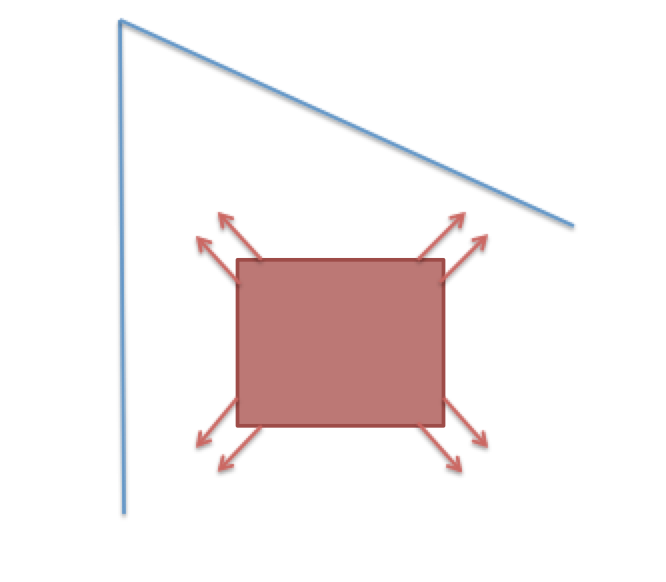
\includegraphics[width=.6\linewidth]{images/flatArea.png}
	\caption{Flat Area}
	\label{fig:flatArea}
\end{minipage}%
\begin{minipage}{.5\textwidth}
	\centering
	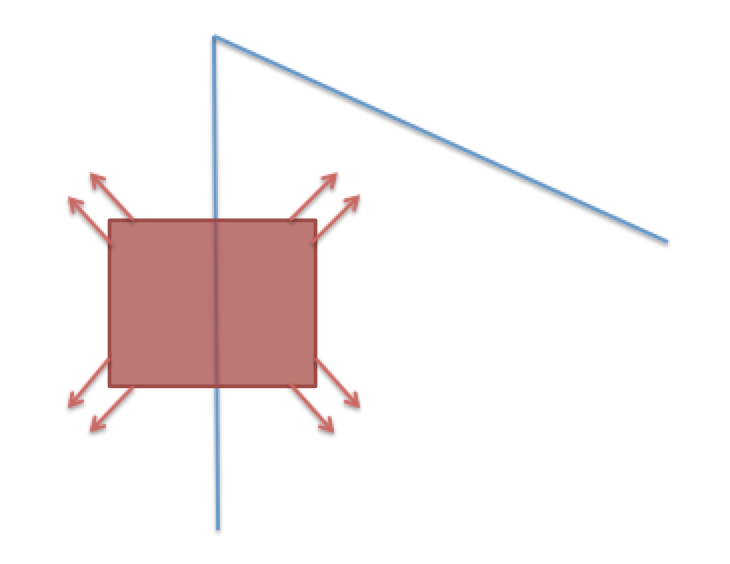
\includegraphics[width=.6\linewidth]{images/edgeArea.png}
	\caption{Edge Area}
	\label{fig:edgeArea}
\end{minipage}
\begin{minipage}{.5\textwidth}
	\centering
	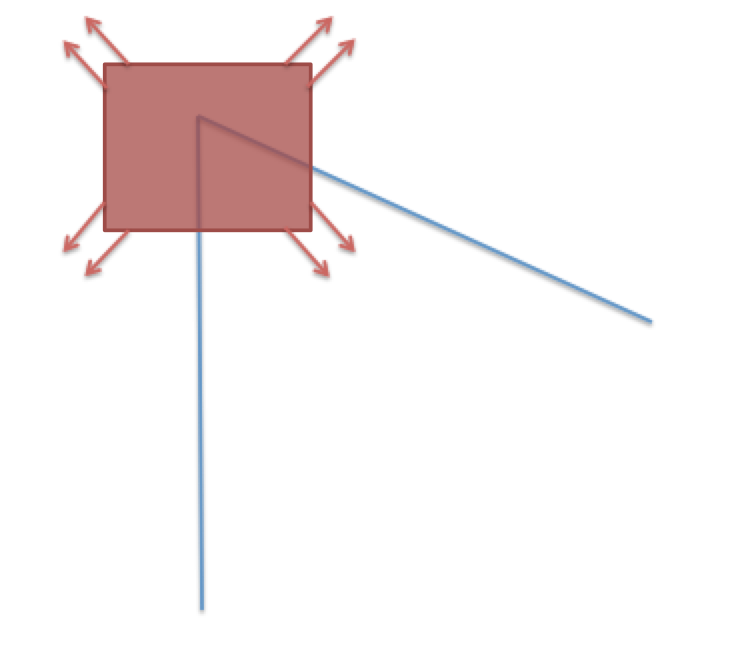
\includegraphics[width=.6\linewidth]{images/cornerArea.png}
	\caption{Corner Area}
	\label{fig:cornerArea}
\end{minipage}
\end{figure}


\section{Scale Invariant Feature Transform}
\subsection{Keypoint localization}
Although the $Harris\ corner\ detection$ algorithm presented in the previous section is immune to rotation transformations of an image, it does not perform well if the image is scaled, because a high intensity change in an area of size $(w, h)$ of an image might vary if the dimensions of the image change, but the size of the area remains the same.\\
Thus, David Lowe, in \cite{siftLowe}, presented a new algorithm for extracting keypoints and computing their descriptors, named $Scale\ Invariant\ Feature\ Transform$.\\
At first, a Gaussian distribution is applied on the analyzed image, which depending of the standard deviation, $\sigma$, blurs the image with a certain amount: $G(x, y) = \frac{1}{2 * \pi * \sigma^2} * e^{-\frac{x^2 + y^2}{2 * \sigma^2}}$.\\
Then, the Laplacian of the image is computed, in order to highlight the regions of rapid intensity changes: $L(x, y) = \frac{\delta^2 I}{\delta x^2} + \frac{\delta^2 I}{\delta y^2}$. Combined with the previous Gaussian filter, we obtain the so called Laplacian of Gaussian: $LoG(x, y) = -\frac{1}{\pi * \sigma^4} * \left(1 - \frac{x^2 + y^2}{2 * \sigma^2}\right) * e^{-\frac{x^2 + y^2}{2 * \sigma^2}}$.\\
Because the $LoG$ has a high computational cost, it is approximated with a Difference of Gaussians, which is a difference of two Gaussians with two different $\sigma$ deviations, representing two different scaled images. The local extrema of the computed $DoG$ are considered potential keypoints.

\subsection{Computing the Descriptors}
Once we have the keypoints, we have to compute a unique fingerprint for a given keypoint, which should be invariant to scaling, rotation and luminance \cite{siftImplementation}.\\
A $16\times16$ window is selected around a keypoint, which is divided into $16$ $4\times4$ blocks. In each of these blocks, the gradient magnitude and orientation is computed for each of the $16$ elements. These gradients are then inserted in a $8$ bin histogram. The histogram is computed using the following principles:
\begin{enumerate}
	\item the gradients are placed in the corresponding bin after their orientation: a gradient in range $0^o-44^o$ is placed in the first bin, a gradient in range $45^o-89^o$ is placed in the second, etc.
	\item the value added to the corresponding bin depends on the gradient magnitude
	\item also, the amount added to the corresponding bin depends on the distance from the keypoint. This is done using a gaussian weighting function
	\item to achieve rotation independence we have to subtract the keypoint's  orientation of the orientation of the histograms.
\end{enumerate}

After this computation, we remain with $16$ $8$ bin histograms, so we get a total of $128$ numbers.
The corresponding descriptors are computed by taking a $16\times16$ neighborhood around the keypoint, and creating a $8$ bin histogram for each sub-block of $4\times4$ size of the initial neighborhood. Thus, a keypoint descriptor will contain $128$ values.
These values are then normalized, and the descriptor of the current keypoint is obtained.

\begin{figure}[ht!]
\centering
\begin{minipage}{.5\textwidth}
	\centering
	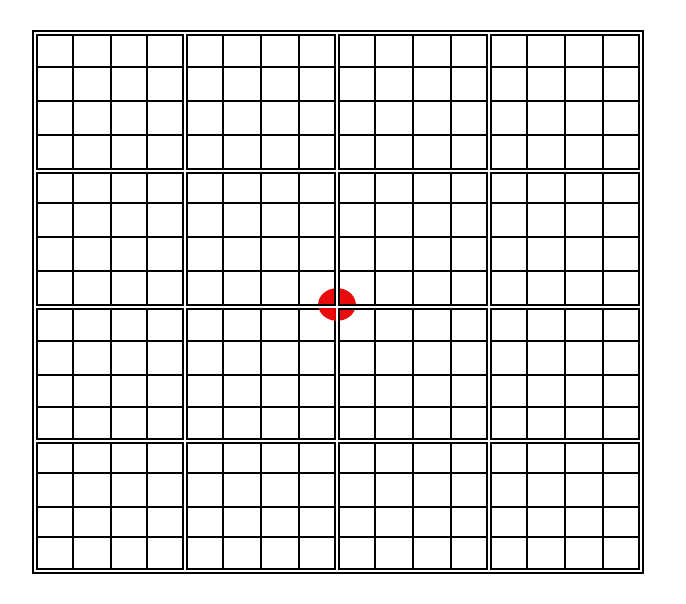
\includegraphics[width=.9\linewidth]{images/spacePartition.png}
	\caption{$16\times16$ window surrounding a\\ keypoint}
	\label{fig:spacePartition}
\end{minipage}%
\begin{minipage}{.5\textwidth}
	\centering
	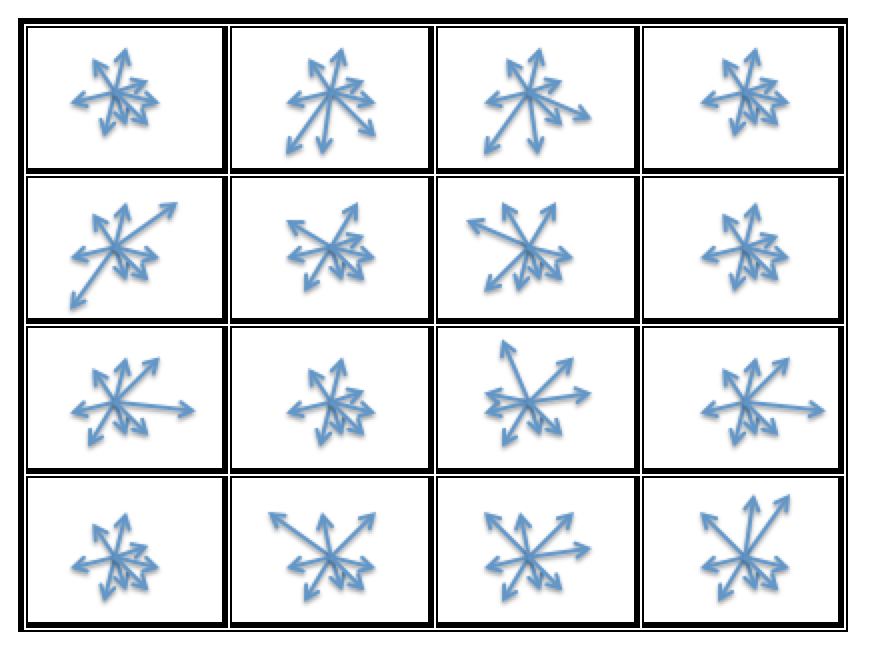
\includegraphics[width=1.1\linewidth]{images/imageGradients.png}
	\caption{Orientation histograms for the\\$4\times4$ window}
	\label{fig:imageGradients}
\end{minipage}
\end{figure}

\section{Speeded Up Robust Features}

SURF (Speeded Up Robust Features) is an algorithm, which was introduced in 2006 as a speeded-up version of SIFT \cite{surf}. Insead of approximating the Laplacian of Gaussian with Difference of Gaussian, as SURF does, It approximates it with the Box Filter.\\
It uses wavelet responses \cite{haarWavelet}, \cite{haarWavelet2} on the X and Y axes to determine orientation assignment, which are plotted in a 2D space and summed up in a sliding window of $60^o$.\\
The wavelet responses are used again to compute the descriptors for the keypoints: a 4-dimensional vector $(\sum{d_x}, \sum{d_y}, \sum{|d_x|}, \sum{|d_y|})$ is computed for each block of size 4x4, thus obtaining a final descriptor of size 64.\\
We were interested in this descriptor, because of its similar performance with the SIFT descriptor, but lower dimension and faster computation.\\

\section{Descriptor Compression}

In \cite{descCompression}, a method is proposed for compressing SIFT and SURF descriptors, reducing their dimension and creating a metric which could be used to compute the distance between two compressed descriptors without requiring their decompression.\\
This method has four parts:
\begin{enumerate}
	\item a matrix which normalizes each row of a certain descriptor
	\item a distance lookup matrix 
	\item a weight vector, which assigns each row of a descriptor a certain weight depending on how much it will contribute to the final distance
	\item a tree coding scheme, similar to Huffman trees, which compresses the descriptors
\end{enumerate}

This is particular interesting for us because it can refuse the dimensionality of our problem, and provide a similar query response with a smaller running time.